\chapter{Fundamentals}

\begin{figure}
	\centering
    \def\svgwidth{0.5\textwidth}
%    \includestandalone[width=\textwidth]{figures/fig/lstmtikz}
    \input{figures/inkscape/aimldl.pdf_tex} %use full path to know the location of pdftex
    \caption{Schema of AI, ML and DL}
    \label{fig:ai_ml_dl}
\end{figure}


\begin{figure}
	\centering
    \def\svgwidth{0.5\textwidth}
%    \includestandalone[width=\textwidth]{figures/fig/lstmtikz}
    \input{figures/inkscape/mlparadigm.pdf_tex} %use full path to know the location of pdftex
    \caption{ML Paradigm. Inspired from \cite{mlparadigm}}
    \label{fig:mlparadigm}
\end{figure}

\begin{figure}
	\centering
    \def\svgwidth{0.8\textwidth}
%    \includestandalone[width=\textwidth]{figures/fig/lstmtikz}
    \input{figures/inkscape/overfitting.pdf_tex} %use full path to know the location of pdftex
    \caption{Relationship between capacity and error. Inspired from
    \cite{Goodfellow-et-al-2016}}
    \label{fig:overfittingunderfitting}
\end{figure}

\begin{figure}
	\begin{center}
	   \def\svgwidth{0.7\textwidth}
%    \includestandalone[width=\textwidth]{figures/fig/lstmtikz}
    \input{figures/inkscape/sigmoid.pdf_tex} %use full path to know the location of pdftex
	\end{center}
    \caption{Activation functions}
    \label{fig:activationfunctions}
\end{figure}

\begin{figure}[h]
	\begin{center}
	   \def\svgwidth{0.8\columnwidth}
%    \includestandalone[width=\textwidth]{figures/fig/lstmtikz}
    \input{figures/inkscape/lstm.pdf_tex} %use full path to know the location of pdftex
	\end{center}
    \caption{lstm from inkscape}
    \label{fig:lstmfrominkscpape}
\end{figure}

\begin{figure}
    \begin{center}
        \includegraphics[width =0.3\textwidth]{figures/inkscape/aimldl.png}
    \end{center}
    \caption{Representing Artificial Intelligence, Machine Learning and Deep Learning as a
    subset of one another.}
    \label{fig:ai_ml_dl}
\end{figure}

\begin{figure}
    \centering
        \def\svgwidth{0.5\textwidth}
        \input{figures/inkscape/multilayer_perceptron.pdf_tex} %use
        \caption{fasdfasf}
    %full path to know the location of pdftex
\end{figure}
\begin{figure}
    \def\svgwidth{0.9\textwidth}
	\begin{center}
        \input{figures/inkscape/inputhiddenoutput.pdf_tex} %use
    %full path to know the location of pdftex
    \end{center}
\end{figure}
\iffalse
\begin{figure}
    \centering
    \begin{subfigure}[t!]{\textwidth}
    \begin{center}
        \input{figures/inkscape/multilayer_perceptron.pdf_tex} %use
    %full path to know the location of pdftex
    \end{center}
        \caption{Lorem ipsum}
    \end{subfigure}\hfill
    \begin{subfigure}[t!]{\textwidth}
        \centering
        \begin{LARGE}
        \input{figures/inkscape/inputhiddenoutput.pdf_tex} %use
        \end{LARGE}
        \caption{Lorem ipsum, lorem ipsum,Lorem ipsum, lorem ipsum,Lorem ipsum}
    \end{subfigure}
    \caption{Caption place holder}
\end{figure}
\fi
\begin{figure}
	\centering
    \includestandalone[width=\textwidth]{figures/fig/SLsetup}
    \caption{Supervised Learning set up}
    \label{fig:SL_setup}
\end{figure}

\begin{figure}
	\centering
    \includestandalone[width=0.5\textwidth]{figures/fig/2d_convolution}
    \caption{Two dimensional convolution}
    \label{fig:2dconv}
\end{figure}

\begin{figure}
	\centering
    \begin{Large}
    \input{figures/inkscape/dropout.pdf_tex}

    \end{Large}
    \caption{Illustrating dropout functionality}
    \label{fig:Dropout_function}
\end{figure}

\begin{figure}
	\centering
    \begin{Large}
        \input{figures/inkscape/minima.pdf_tex}

    \end{Large}
    \caption{Finding the stochastic gradient descent}
    \label{fig:gradientdescent}
\end{figure}

\begin{figure}
	\centering
        \def\svgwidth{0.8\textwidth}

        \input{figures/inkscape/lossfunction.pdf_tex}

    \caption{Loss function}
    \label{fig:loss function}
\end{figure}

\begin{figure}
	\centering
        \def\svgwidth{0.81\textwidth}

        \input{figures/inkscape/optimizer.pdf_tex}

    \caption{With optimizer}
    \label{fig:withoptimizer}
\end{figure}


\begin{figure}
	\centering
        \def\svgwidth{0.8\textwidth}
\begin{tiny}
        \input{figures/inkscape/simplernn.pdf_tex}

\end{tiny}

    \caption{simple rnn}
    \label{fig:rnn}
\end{figure}


